\documentclass[aspectratio=169,11pt]{beamer}
\usetheme{Madrid}
\usecolortheme{default}

% Fix navigation symbols overflow in 16:9
\setbeamertemplate{navigation symbols}{}
\setbeamertemplate{footline}{
    \leavevmode%
    \hbox{%
        \begin{beamercolorbox}[wd=.333333\paperwidth,ht=2.25ex,dp=1ex,center]{author in head/foot}%
            \usebeamerfont{author in head/foot}\insertshortauthor
        \end{beamercolorbox}%
        \begin{beamercolorbox}[wd=.333333\paperwidth,ht=2.25ex,dp=1ex,center]{title in head/foot}%
            \usebeamerfont{title in head/foot}\insertshorttitle
        \end{beamercolorbox}%
        \begin{beamercolorbox}[wd=.333333\paperwidth,ht=2.25ex,dp=1ex,right]{date in head/foot}%
            \usebeamerfont{date in head/foot}\insertshortdate{}\hspace*{2em}
            \insertframenumber{} / \inserttotalframenumber\hspace*{2ex}
        \end{beamercolorbox}}%
    \vskip0pt%
}

% Custom colors - Labor/Work theme
\definecolor{laborblue}{RGB}{0,90,156}
\definecolor{laborgreen}{RGB}{46,139,87}
\definecolor{labororange}{RGB}{210,105,30}
\definecolor{laborpurple}{RGB}{102,51,153}
\definecolor{labored}{RGB}{178,34,34}
\definecolor{laborgold}{RGB}{184,134,11}

\setbeamercolor{structure}{fg=laborblue}
\setbeamercolor{title}{fg=white,bg=laborblue}
\setbeamercolor{frametitle}{fg=white,bg=laborblue}
\setbeamercolor{block title}{fg=white,bg=laborblue}
\setbeamercolor{block body}{bg=laborblue!10}

% Packages
\usepackage{tikz}
\usetikzlibrary{shapes,arrows,positioning,decorations.pathreplacing,calc,fit}
\usepackage{booktabs}
\usepackage{tcolorbox}
\tcbuselibrary{skins,breakable}

% Custom boxes
\newtcolorbox{conceptbox}[1][]{
    colback=laborblue!5,
    colframe=laborblue,
    fonttitle=\bfseries,
    title=#1
}

\newtcolorbox{probox}[1][]{
    colback=laborgreen!5,
    colframe=laborgreen!80!black,
    fonttitle=\bfseries,
    title=#1
}

\newtcolorbox{objectionbox}[1][]{
    colback=labored!5,
    colframe=labored!80!black,
    fonttitle=\bfseries,
    title=#1
}

\newtcolorbox{casestudybox}[1][]{
    colback=labororange!10,
    colframe=labororange!80!black,
    fonttitle=\bfseries,
    title=#1
}

\newtcolorbox{quotebox}[1][]{
    colback=gray!5,
    colframe=gray!50,
    fonttitle=\bfseries,
    title=#1
}

\newtcolorbox{discussionbox}[1][]{
    colback=laborpurple!5,
    colframe=laborpurple!80!black,
    fonttitle=\bfseries,
    title=#1
}

% Title information
\title[AI and Human Labor]{AI and the Future of Human Labor}
\subtitle{Work, Art, and Human Flourishing in the Age of Automation}
\author{Computing and AI Ethics}
\institute{Rochester Community and Technical College}
\date{}

\begin{document}

% Slide 1: Title
\begin{frame}
\titlepage
\end{frame}

% Slide 2: Central Questions
\begin{frame}{Central Questions}
\begin{itemize}
    \item What is work, and why does it matter to human life?
    \item What makes work \emph{meaningful}?
    \item How might AI transform---or threaten---the value we derive from work?
    \item Can AI do ``real'' work, especially creative work?
\end{itemize}

\vspace{0.3em}
\begin{alertblock}{The Stakes}
AI doesn't just threaten jobs---it threatens the human activities through which we find meaning, develop skills, and express ourselves.
\end{alertblock}
\end{frame}

%%% PART I: WHAT IS WORK? %%%
\section{Part I: What Is Work?}

% Slide 3: Arendt's Distinction
\begin{frame}{Arendt's Distinction: Labor vs.\ Work vs.\ Action}
\begin{columns}[T]
\begin{column}{0.55\textwidth}
Hannah Arendt, \emph{The Human Condition} (1958):

\vspace{0.2em}
\textbf{Labor} (\emph{animal laborans}): Cyclical activities for survival; leaves nothing behind; consumed as quickly as produced.

\vspace{0.2em}
\textbf{Work} (\emph{homo faber}): Creates durable objects that outlast the maker; builds a ``world'' of human artifice.

\vspace{0.2em}
\textbf{Action}: Disclosing oneself through deeds in the public sphere; politics, speech, initiative.
\end{column}
\begin{column}{0.42\textwidth}
\begin{center}
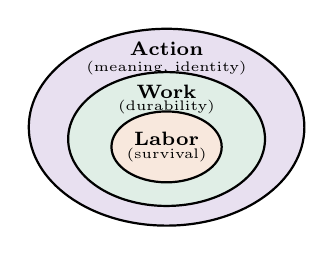
\begin{tikzpicture}[scale=0.5]
    % Three nested rounded rectangles
    \draw[thick, fill=laborpurple!15] (0,0) ellipse (3.5cm and 2.5cm);
    \node[font=\scriptsize] at (0,2) {\textbf{Action}};
    \node[font=\tiny] at (0,1.5) {(meaning, identity)};
    
    \draw[thick, fill=laborgreen!15] (0,-0.3) ellipse (2.5cm and 1.7cm);
    \node[font=\scriptsize] at (0,0.9) {\textbf{Work}};
    \node[font=\tiny] at (0,0.5) {(durability)};
    
    \draw[thick, fill=labororange!15] (0,-0.5) ellipse (1.4cm and 0.9cm);
    \node[font=\scriptsize] at (0,-0.3) {\textbf{Labor}};
    \node[font=\tiny] at (0,-0.7) {(survival)};
\end{tikzpicture}
\end{center}
{\scriptsize Increasing durability and meaning}
\end{column}
\end{columns}
\end{frame}

% Slide 4: Why the Distinction Matters
\begin{frame}{Why This Distinction Matters}
\begin{quotebox}[Arendt on Labor]
\small
``It is indeed the mark of all laboring that it leaves nothing behind, that the result of its effort is almost as quickly consumed as the effort is spent.''
\end{quotebox}

\vspace{0.2em}
\textbf{Labor} is necessary but futile---it never ends, produces nothing lasting.

\vspace{0.2em}
\textbf{Work} creates meaning by leaving something in the world: a table, a book, a building, a work of art.

\vspace{0.2em}
\textbf{Arendt's worry}: Modernity reduces everything to labor---even art becomes ``content'' to be consumed. We become trapped in cycles of production and consumption with no lasting achievement.
\end{frame}

% Slide 5: Historical Anxiety
\begin{frame}{Historical Anxiety: Technology Replacing Work with Labor}
This worry is old! Technology has long threatened to eliminate \emph{craft} while preserving \emph{toil}.

\vspace{0.2em}
\begin{itemize}
    \item \textbf{Luddites (1811)}: Textile workers smashing machines that ``deskilled'' their craft
    \item \textbf{Arendt (1958)}: Worried capitalism and automation would reduce all work to labor
\end{itemize}

\vspace{0.2em}
\begin{casestudybox}[Chaplin's \emph{Modern Times} (1936)]
\scriptsize
The Tramp becomes a literal cog in the machine---tightening bolts on an assembly line until he has a breakdown. The famous ``feeding machine'' scene: technology optimizes labor but dehumanizes the worker. The film captures the fear that technology doesn't eliminate toil---it eliminates craft.
\end{casestudybox}
\end{frame}

% Slide 6: Work Broadly Construed
\begin{frame}{Work Broadly Construed: Including Artistic Creation}
For Arendt, \textbf{artworks are the most durable products of work}---they persist across generations and build the cultural world.

\vspace{0.3em}
\textbf{Creative work} = paradigm case of meaningful work:
\begin{itemize}
    \item Involves vision, planning, skill development
    \item Leaves something lasting in the world
    \item Expresses the maker's identity and values
\end{itemize}

\vspace{0.3em}
\textbf{Other examples}: Scientific discovery, engineering feats, philosophical writing, craft traditions.

\vspace{0.3em}
\textbf{Key insight}: Work isn't just about earning money---it's about \emph{making something} that matters.
\end{frame}

% Slide 7: Psychology of Meaningful Work
\begin{frame}{The Psychology of Meaningful Work}
\begin{columns}[T]
\begin{column}{0.48\textwidth}
\textbf{Self-Determination Theory} (Ryan \& Deci):

Three basic psychological needs satisfied by meaningful work:

\vspace{0.2em}
\begin{enumerate}
    \item \textbf{Autonomy}: Sense of volition and choice
    \item \textbf{Competence}: Feeling effective and capable
    \item \textbf{Relatedness}: Connection to others
\end{enumerate}

\vspace{0.2em}
Research shows: Satisfying these needs $\rightarrow$ well-being, engagement, performance.
\end{column}
\begin{column}{0.48\textwidth}
\begin{table}[h]
\centering
\scriptsize
\begin{tabular}{@{}p{1.8cm}p{3.5cm}@{}}
\toprule
\textbf{Need} & \textbf{Workplace Example} \\
\midrule
Autonomy & Flexible scheduling, input on methods \\
\addlinespace
Competence & Skill development, mastery experiences \\
\addlinespace
Relatedness & Team collaboration, mentorship \\
\bottomrule
\end{tabular}
\end{table}
\end{column}
\end{columns}
\end{frame}

% Slide 8: Non-Monetary Value of Work
\begin{frame}{Beyond Money: The Non-Monetary Value of Work}
Work provides:
\begin{itemize}
    \item \textbf{Identity and self-expression}: ``What do you do?''
    \item \textbf{Structure and purpose}: Organizing time, setting goals
    \item \textbf{Social connection}: Colleagues, professional communities
    \item \textbf{Contribution}: Feeling useful, making a difference
    \item \textbf{Mastery and growth}: Developing skills over time
\end{itemize}

\vspace{0.2em}
\textbf{Research finding}: Unemployed people suffer psychologically even when financially secure.

\vspace{0.2em}
\begin{discussionbox}[Discussion Question]
\small
If you won the lottery tomorrow, would you still work? Why or why not?
\end{discussionbox}
\end{frame}

% Slide 9: Meaningful Work as Beneficence
\begin{frame}{Meaningful Work and Beneficence}
\begin{conceptbox}[Four Pathways to Meaningful Work]
\small
(Martela \& Ryan, 2018): Autonomy + Competence + Relatedness + \textbf{Beneficence} (helping others)
\end{conceptbox}

\vspace{0.2em}
Work feels meaningful when it \textbf{contributes to something beyond ourselves}.

\vspace{0.2em}
This explains why ``bullshit jobs'' (Graeber) feel soul-crushing even when well-paid---they lack purpose and contribution.

\vspace{0.2em}
\begin{objectionbox}[Objection]
\small
Not all jobs feel meaningful---many are tedious, exploitative, or pointless. Should we idealize work?
\end{objectionbox}
\end{frame}

% Slide 10: Transition
\begin{frame}{Transition: Why Does This Matter for AI?}
AI threatens to transform work in fundamental ways:

\vspace{0.3em}
\begin{enumerate}
    \item \textbf{Replacement}: AI eliminates jobs entirely
    \item \textbf{Deskilling}: AI replaces work with ``mere labor''
    \item \textbf{Augmentation}: AI handles labor so humans can do \emph{more/better} work
\end{enumerate}

\vspace{0.3em}
\textbf{The stakes}: Not just economic (lost wages), but existential---what happens to human meaning and flourishing when work disappears or degrades?

\vspace{0.3em}
Before examining AI's impact, we need to understand \emph{why} meaningful work is ethically valuable.
\end{frame}

%%% PART II: WHY IS MEANINGFUL WORK ETHICALLY VALUABLE? %%%
\section{Part II: Why Is Meaningful Work Ethically Valuable?}

% Slide 11: Three Ethical Frameworks
\begin{frame}{Three Ethical Perspectives on Work}
\begin{center}
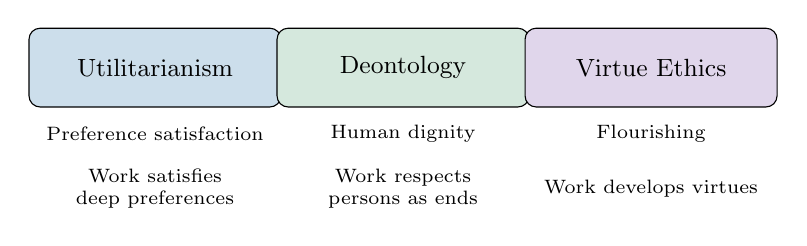
\begin{tikzpicture}[scale=0.7, every node/.style={font=\small}]
    % Three columns
    \node[draw, rounded corners, fill=laborblue!20, minimum width=3.2cm, minimum height=1cm] (util) at (-4.5,0) {Utilitarianism};
    \node[draw, rounded corners, fill=laborgreen!20, minimum width=3.2cm, minimum height=1cm] (deont) at (0,0) {Deontology};
    \node[draw, rounded corners, fill=laborpurple!20, minimum width=3.2cm, minimum height=1cm] (virtue) at (4.5,0) {Virtue Ethics};
    
    % Key concepts
    \node[font=\scriptsize, text width=3cm, align=center] at (-4.5,-1.2) {Preference satisfaction};
    \node[font=\scriptsize, text width=3cm, align=center] at (0,-1.2) {Human dignity};
    \node[font=\scriptsize, text width=3cm, align=center] at (4.5,-1.2) {Flourishing};
    
    % Work implications
    \node[font=\scriptsize, text width=3cm, align=center] at (-4.5,-2.2) {Work satisfies deep preferences};
    \node[font=\scriptsize, text width=3cm, align=center] at (0,-2.2) {Work respects persons as ends};
    \node[font=\scriptsize, text width=3cm, align=center] at (4.5,-2.2) {Work develops virtues};
\end{tikzpicture}
\end{center}

\vspace{0.3em}
Each framework offers distinct reasons for valuing meaningful work---and for worrying about AI's impact on it.
\end{frame}

% Slide 12: Preference Utilitarianism
\begin{frame}{Preference Utilitarianism: Work and Well-Being}
\begin{probox}[Utilitarian Argument for Meaningful Work]
\small
\begin{enumerate}
    \item We should maximize preference satisfaction.
    \item Meaningful work satisfies deep, enduring human preferences (for autonomy, mastery, purpose, contribution).
    \item Loss of meaningful work frustrates these preferences, causing suffering.
    \item Therefore, we have utilitarian reasons to preserve meaningful work.
\end{enumerate}
\end{probox}

\vspace{0.2em}
\textbf{Empirical support}: Work satisfaction strongly correlates with life satisfaction. Unemployment causes psychological harm beyond income loss.
\end{frame}

% Slide 13: Utilitarian Complications
\begin{frame}{Utilitarian Complications}
But utilitarians must weigh \emph{all} preferences:
\begin{itemize}
    \item Consumers prefer cheaper goods (AI can provide)
    \item Society prefers efficient production
    \item Shareholders prefer higher profits
    \item Workers displaced by AI suffer, but others may benefit
\end{itemize}

\vspace{0.2em}
\begin{objectionbox}[Objection]
\small
What if AI-produced goods satisfy more preferences overall? Shouldn't we accept worker displacement for the greater good?
\end{objectionbox}

\vspace{0.2em}
\textbf{Response}: Consider the \emph{depth and durability} of work-related preferences vs.\ consumer preferences. Losing meaningful work may cause more suffering than slightly more expensive goods.
\end{frame}

% Slide 14: Deontology
\begin{frame}{Deontology: Work and Human Dignity}
\begin{probox}[Deontological Argument for Meaningful Work]
\small
\begin{enumerate}
    \item Persons must be treated as ends in themselves, never merely as means (Kant).
    \item Meaningful work treats persons as ends: it develops their capacities, respects their autonomy, recognizes them as rational agents.
    \item Reducing work to mere labor treats persons as means: cogs in a machine, instruments of production.
    \item Therefore, we have duties to preserve meaningful work.
\end{enumerate}
\end{probox}

\vspace{0.2em}
Work that respects dignity allows for autonomous choice, develops rational capacities, and recognizes workers as persons with inherent worth.
\end{frame}

% Slide 15: Deontological Complications
\begin{frame}{Deontological Complications}
\begin{itemize}
    \item Does anyone have a \emph{right} to meaningful work?
    \item Whose \emph{duty} is it to provide meaningful work?
    \item What about work that is necessary but not meaningful?
\end{itemize}

\vspace{0.2em}
\begin{objectionbox}[Objection]
\small
Kantian autonomy is about rational self-legislation, not job satisfaction. You can be autonomous even in tedious work.
\end{objectionbox}

\vspace{0.2em}
\textbf{Response}: But work conditions can enable or undermine our capacity for rational agency. Surveillance, algorithmic management, and deskilling reduce workers' ability to exercise judgment and make meaningful choices.
\end{frame}

% Slide 16: Virtue Ethics
\begin{frame}{Virtue Ethics: Work and Human Flourishing}
\begin{probox}[Virtue Ethics Argument for Meaningful Work]
\small
\begin{enumerate}
    \item Human flourishing (\emph{eudaimonia}) requires exercising virtues through practices (Aristotle, MacIntyre).
    \item Meaningful work is a practice with ``internal goods''---excellences specific to the activity itself.
    \item AI that eliminates such practices removes opportunities for developing virtue.
    \item Therefore, we have virtue-ethical reasons to preserve meaningful work.
\end{enumerate}
\end{probox}

\vspace{0.2em}
Work as a site for developing: practical wisdom (\emph{phronesis}), craftsmanship, perseverance, justice, courage.

\vspace{0.2em}
MacIntyre's distinction: \textbf{Internal goods} (excellence in the practice) vs.\ \textbf{external goods} (money, status).
\end{frame}

% Slide 17: Summary Table
\begin{frame}{Summary: Three Perspectives on Meaningful Work}
\begin{table}[h]
\centering
\scriptsize
\begin{tabular}{@{}p{2.3cm}p{2.8cm}p{3.2cm}p{3.5cm}@{}}
\toprule
\textbf{Framework} & \textbf{Key Value} & \textbf{Why Work Matters} & \textbf{Concern About AI} \\
\midrule
Utilitarianism & Preference satisfaction & Work satisfies deep preferences & Must weigh against consumer preferences \\
\addlinespace
Deontology & Human dignity & Work respects persons as ends & Deskilling treats workers as means \\
\addlinespace
Virtue Ethics & Flourishing & Work develops virtues & Automation eliminates virtuous practice \\
\bottomrule
\end{tabular}
\end{table}

\vspace{0.2em}
\textbf{Key insight}: All three frameworks give us reasons to care about the \emph{quality} of work, not just whether jobs exist.
\end{frame}

%%% PART III: HOW MIGHT AI BE DEPLOYED? %%%
\section{Part III: How Might AI Transform Work?}

% Slide 18: Three Scenarios
\begin{frame}{Three Scenarios for AI and Work}
\begin{center}
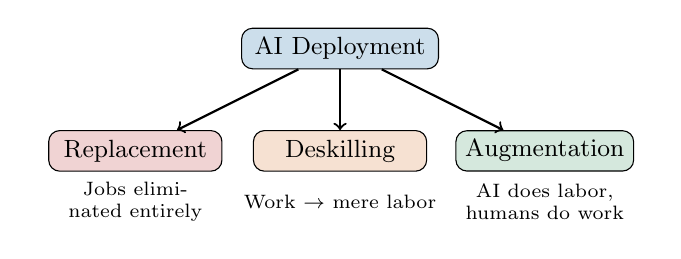
\begin{tikzpicture}[scale=0.65, every node/.style={font=\small}]
    % Root
    \node[draw, rounded corners, fill=laborblue!20, minimum width=2.5cm] (ai) at (0,2) {AI Deployment};
    
    % Three branches
    \node[draw, rounded corners, fill=labored!20, minimum width=2.2cm] (replace) at (-4,0) {Replacement};
    \node[draw, rounded corners, fill=labororange!20, minimum width=2.2cm] (deskill) at (0,0) {Deskilling};
    \node[draw, rounded corners, fill=laborgreen!20, minimum width=2.2cm] (augment) at (4,0) {Augmentation};
    
    % Arrows
    \draw[->, thick] (ai) -- (replace);
    \draw[->, thick] (ai) -- (deskill);
    \draw[->, thick] (ai) -- (augment);
    
    % Descriptions
    \node[font=\scriptsize, text width=2.5cm, align=center] at (-4,-1) {Jobs eliminated entirely};
    \node[font=\scriptsize, text width=2.5cm, align=center] at (0,-1) {Work $\rightarrow$ mere labor};
    \node[font=\scriptsize, text width=2.5cm, align=center] at (4,-1) {AI does labor, humans do work};
\end{tikzpicture}
\end{center}

\vspace{0.2em}
These aren't mutually exclusive---different jobs face different futures. The outcome depends on \emph{how we choose to deploy AI}.
\end{frame}

% Slide 19: Scenario 1 - Replacement
\begin{frame}{Scenario 1: Job Replacement}
Some jobs will simply disappear:
\begin{itemize}
    \item Toll booth operators $\rightarrow$ electronic tolling
    \item Bank tellers $\rightarrow$ ATMs and apps
    \item Travel agents $\rightarrow$ online booking
    \item Cashiers $\rightarrow$ self-checkout
    \item Data entry clerks $\rightarrow$ automated processing
\end{itemize}

\vspace{0.2em}
\textbf{Scale}: McKinsey estimates 400--800 million workers could be displaced globally by 2030.

\vspace{0.2em}
This is the most \emph{visible} AI threat---but perhaps not the most insidious.
\end{frame}

% Slide 20: Replacement - Ethical Analysis
\begin{frame}{Replacement: Ethical Analysis}
\begin{itemize}
    \item \textbf{Utilitarian}: Displaced workers suffer, but consumers and shareholders may benefit. Net calculation unclear.
    \item \textbf{Deontological}: Workers aren't mere instruments---displacement without support violates dignity.
    \item \textbf{Virtue ethics}: Loss of practice means loss of opportunity for flourishing.
\end{itemize}

\vspace{0.2em}
\begin{casestudybox}[Case Study: Trucking]
\scriptsize
3.5 million U.S. truck drivers face potential displacement from autonomous vehicles. Trucking provides middle-class income without college degree. Communities built around truck stops and logistics. What happens to these workers and communities?
\end{casestudybox}
\end{frame}

% Slide 21: Scenario 2 - Deskilling
\begin{frame}{Scenario 2: Deskilling (Work $\rightarrow$ Labor)}
More insidious than replacement: AI doesn't eliminate jobs but \textbf{strips them of meaning}.

\vspace{0.2em}
\textbf{Floridi's ``enveloping''}: We adapt work environments to AI's limitations.

\vspace{0.2em}
Workers become:
\begin{itemize}
    \item Supervisors of AI systems they don't understand
    \item Button-pushers confirming AI decisions
    \item Data-entry clerks feeding AI systems
    \item ``Human in the loop'' for liability purposes only
\end{itemize}

\vspace{0.2em}
The job \emph{exists} but the \emph{craft} is gone. This is Arendt's nightmare: work reduced to labor.
\end{frame}

% Slide 22: Deskilling Examples
\begin{frame}{Examples of Deskilling}
\begin{table}[h]
\centering
\scriptsize
\begin{tabular}{@{}p{2cm}p{3.2cm}p{3.2cm}p{3.2cm}@{}}
\toprule
\textbf{Profession} & \textbf{Before AI} & \textbf{After AI} & \textbf{What's Lost} \\
\midrule
Radiologist & Interprets images using expertise & Reviews AI-flagged cases & Diagnostic skill \\
\addlinespace
Writer & Crafts prose through revision & Edits AI drafts & Voice, creative process \\
\addlinespace
Designer & Envisions and creates & Tweaks AI outputs & Artistic vision \\
\addlinespace
Programmer & Architects solutions & Prompts and debugs AI & Problem-solving craft \\
\bottomrule
\end{tabular}
\end{table}

\vspace{0.2em}
In each case: The worker may still have a ``job,'' but the meaningful \emph{work} has been hollowed out.
\end{frame}

% Slide 23: Deskilling - A Deeper Worry
\begin{frame}{Deskilling: A Deeper Worry}
Deskilled workers may keep jobs but lose:
\begin{itemize}
    \item \textbf{Autonomy}: AI makes decisions, workers execute
    \item \textbf{Competence}: Skills atrophy from disuse
    \item \textbf{Relatedness}: Less collaboration, more algorithmic management
\end{itemize}

\vspace{0.2em}
\begin{casestudybox}[Case Study: Amazon Warehouses]
\scriptsize
Workers tracked by wristbands monitoring movements. Algorithmically determined pace---no human judgment about workflow. Bathroom breaks timed and penalized. Workers describe feeling like ``robots'' or ``appendages to machines.'' Jobs exist, but are they meaningful work?
\end{casestudybox}
\end{frame}

% Slide 24: Deskilling - Ethical Analysis
\begin{frame}{Deskilling: Ethical Analysis}
\begin{itemize}
    \item \textbf{Utilitarian}: Workers may be employed but deeply unsatisfied; preferences for autonomy and mastery frustrated.
    \item \textbf{Deontological}: Treating workers as mere instruments of production---means rather than ends.
    \item \textbf{Virtue ethics}: No opportunity to develop excellence; flourishing systematically undermined.
\end{itemize}

\vspace{0.3em}
\textbf{All three frameworks converge}: Deskilling is ethically problematic, even when it preserves employment.

\vspace{0.3em}
\begin{alertblock}{Key Insight}
``Having a job'' is not the same as ``having meaningful work.''
\end{alertblock}
\end{frame}

% Slide 25: Scenario 3 - Augmentation
\begin{frame}{Scenario 3: Augmentation (AI Does Labor, Humans Do Work)}
\textbf{Optimistic vision}: AI handles tedious tasks, freeing humans for creative, meaningful work.

\vspace{0.3em}
\textbf{Examples}:
\begin{itemize}
    \item AI transcribes meetings $\rightarrow$ professionals focus on strategy
    \item AI handles routine legal research $\rightarrow$ lawyers focus on argumentation
    \item AI grades routine assignments $\rightarrow$ teachers focus on mentorship
    \item AI generates rough drafts $\rightarrow$ writers focus on voice and revision
\end{itemize}

\vspace{0.3em}
AI as Steve Jobs's ``bicycle for the mind''---amplifying human capabilities rather than replacing them.
\end{frame}

% Slide 26: The Augmentation Dream
\begin{frame}{The Augmentation Dream}
\textbf{Historical precedent}: Technology has augmented work before.
\begin{itemize}
    \item Spreadsheets didn't eliminate accountants---freed them for analysis
    \item Spell-checkers didn't eliminate writers---freed them from proofreading
    \item CAD software didn't eliminate architects---enabled more complex designs
\end{itemize}

\vspace{0.2em}
\begin{casestudybox}[Case Study: GitHub Copilot]
\scriptsize
AI coding assistant that suggests code completions. Programmers report: less time on boilerplate, more time on architecture and design. The \emph{tedious} parts automated; the \emph{creative} parts preserved. Is this the future of human-AI collaboration?
\end{casestudybox}
\end{frame}

% Slide 27: Is Augmentation Inevitable?
\begin{frame}{But Is Augmentation Inevitable?}
\begin{objectionbox}[Objection]
\small
``Augmentation is just a pit stop on the way to replacement. Today's copilot is tomorrow's autopilot.''
\end{objectionbox}

\vspace{0.2em}
\textbf{Market incentives} often favor replacement over augmentation:
\begin{itemize}
    \item Cheaper to replace workers than to augment them
    \item Augmentation requires investment in training, restructuring
    \item Historical pattern: Benefits of automation accrue to capital, not labor
\end{itemize}

\vspace{0.2em}
\textbf{Augmentation doesn't happen automatically}---it requires deliberate choices by employers, policymakers, and society.
\end{frame}

% Slide 28: Policy Implications
\begin{frame}{Policy Implications}
If we want augmentation rather than replacement or deskilling, we need deliberate intervention:

\vspace{0.2em}
\begin{itemize}
    \item \textbf{Tax structures} that favor augmentation over replacement
    \item \textbf{Investment} in worker training and reskilling
    \item \textbf{Regulations} requiring human oversight in certain domains
    \item \textbf{Safety nets} (UBI, universal basic services) for transitions
    \item \textbf{Worker voice} in decisions about AI deployment
\end{itemize}

\vspace{0.2em}
\begin{discussionbox}[Discussion Question]
\small
What policies would best preserve meaningful work while allowing society to benefit from AI?
\end{discussionbox}
\end{frame}

% Slide 29: Media Example - WALL-E
\begin{frame}{Media Example: \emph{WALL-E} (2008)}
\begin{columns}[T]
\begin{column}{0.55\textwidth}
Pixar's vision of fully automated leisure:
\begin{itemize}
    \item Humans on the Axiom have all labor automated
    \item Result: Atrophied bodies, passive consumption, no meaningful activity
    \item Ironically, WALL-E (the robot) has more ``humanity''---curiosity, care, relationships
\end{itemize}

\vspace{0.2em}
\textbf{Message}: A life without work (labor or work) isn't liberation---it's dehumanization.
\end{column}
\begin{column}{0.42\textwidth}
\begin{discussionbox}[Discussion]
\scriptsize
Is the Axiom a utopia or dystopia? The humans have no material wants---but are they flourishing?
\end{discussionbox}

\vspace{0.3em}
\textbf{Connection to Arendt}: Without work, there's nothing durable to ground human existence. Only consumption remains.
\end{column}
\end{columns}
\end{frame}

% Slide 30: Media Examples - Classic Films
\begin{frame}{Media Examples: \emph{Metropolis} and \emph{Modern Times}}
\begin{columns}[T]
\begin{column}{0.48\textwidth}
\textbf{\emph{Metropolis}} (1927):
\begin{itemize}
    \item Workers as literal cogs in machines
    \item Robot Maria as false liberation
    \item Class division between thinkers and workers
\end{itemize}
\end{column}
\begin{column}{0.48\textwidth}
\textbf{\emph{Modern Times}} (1936):
\begin{itemize}
    \item Chaplin's Tramp loses himself to assembly-line labor
    \item ``Feeding machine'' scene
    \item Technology optimizes labor but destroys humanity
\end{itemize}
\end{column}
\end{columns}

\vspace{0.3em}
\textbf{Both films}: Technology doesn't free workers---it can enslave them. The \emph{design} of technology matters as much as the technology itself.

\vspace{0.2em}
These anxieties from the early 20th century anticipate our AI concerns today.
\end{frame}

%%% PART IV: OTHER VALUES MATTER TOO %%%
\section{Part IV: Meaningful Work Isn't the Only Value}

% Slide 31: Other Values
\begin{frame}{Other Values Matter Too}
We shouldn't fetishize work---other goods matter:
\begin{itemize}
    \item \textbf{Leisure and rest}: Time for family, friends, hobbies, contemplation
    \item \textbf{Health and safety}: Dangerous or unhealthy work isn't automatically good
    \item \textbf{Consumer welfare}: Cheaper, better goods improve lives
    \item \textbf{Environmental sustainability}: Some work harms the planet
    \item \textbf{Care work}: Often unpaid, often undervalued
\end{itemize}

\vspace{0.2em}
Even Arendt valued \emph{action} (politics, civic engagement) over work. Work is important but not supreme.
\end{frame}

% Slide 32: Bullshit Jobs
\begin{frame}{The Problem of ``Bullshit Jobs''}
\begin{conceptbox}[David Graeber's Thesis]
\small
Many jobs are pointless---even workers know it. These ``bullshit jobs'' provide income but no meaning.
\end{conceptbox}

\vspace{0.2em}
\textbf{Graeber's categories}: Box-tickers, task-masters, goons, duct-tapers, flunkies.

\vspace{0.2em}
If a job doesn't need to exist, is preserving it really valuable?

\vspace{0.2em}
\textbf{Implication}: AI eliminating genuinely pointless jobs might be \emph{good}.

\vspace{0.2em}
\begin{objectionbox}[Objection]
\small
But even ``bullshit'' jobs provide income, structure, and social connection. Eliminating them without alternatives causes harm.
\end{objectionbox}
\end{frame}

% Slide 33: Balancing Values
\begin{frame}{Balancing Values Across Frameworks}
\begin{table}[h]
\centering
\scriptsize
\begin{tabular}{@{}p{2.5cm}p{4.5cm}p{4.5cm}@{}}
\toprule
\textbf{Framework} & \textbf{Values Beyond Work} & \textbf{How to Balance} \\
\midrule
Utilitarianism & All preferences count equally & Weigh worker satisfaction against consumer benefit \\
\addlinespace
Deontology & Dignity in all domains & Respect persons as workers AND consumers \\
\addlinespace
Virtue Ethics & Leisure, contemplation, relationships & Work is one site of flourishing, not the only one \\
\bottomrule
\end{tabular}
\end{table}

\vspace{0.2em}
\textbf{Key insight}: The goal isn't to preserve all jobs---it's to preserve and create conditions for human flourishing, which includes but isn't limited to meaningful work.
\end{frame}

% Slide 34: A Balanced View
\begin{frame}{A Balanced View}
\textbf{Don't assume} all AI impact on work is bad.

\textbf{Don't assume} all AI impact on work is good.

\vspace{0.3em}
\textbf{Ask about any AI deployment}:
\begin{enumerate}
    \item Does it preserve or undermine \textbf{autonomy}?
    \item Does it enable or prevent \textbf{skill development}?
    \item Does it contribute to or detract from \textbf{human flourishing}?
    \item How are \textbf{benefits and burdens distributed}?
    \item What \textbf{alternatives} are available to displaced workers?
\end{enumerate}
\end{frame}

%%% PART V: CAN AI DO "REAL" WORK? %%%
\section{Part V: Can AI Do ``Real'' Work?}

% Slide 35: AI Creativity
\begin{frame}{The Question of AI Creativity}
AI can now generate:
\begin{itemize}
    \item \textbf{Images}: DALL-E, Midjourney, Stable Diffusion
    \item \textbf{Music}: Suno, AIVA, various generators
    \item \textbf{Writing}: GPT, Claude, and other LLMs
    \item \textbf{Code}: GitHub Copilot, Cursor, coding assistants
\end{itemize}

\vspace{0.3em}
\textbf{Questions}:
\begin{itemize}
    \item Is this ``work'' in Arendt's sense? Does it create lasting value?
    \item Or is it sophisticated pattern-matching that produces ephemeral content?
    \item Can AI \emph{originate} anything, or only recombine?
\end{itemize}
\end{frame}

% Slide 36: Arguments Against AI Art
\begin{frame}{Arguments That AI Art Isn't ``Real'' Work}
\begin{itemize}
    \item \textbf{No intention}: AI has no vision, nothing to ``say''
    \item \textbf{No lived experience}: Art expresses human life; AI has none
    \item \textbf{No struggle}: Mastery requires effort; AI produces effortlessly
    \item \textbf{No authenticity}: AI recombines training data, doesn't originate
    \item \textbf{No mortality}: Art derives meaning from finite human life
\end{itemize}

\vspace{0.2em}
\begin{objectionbox}[Objection]
\small
``AI art is just remixing---but isn't all human art influenced by predecessors? What makes human creativity fundamentally different?''
\end{objectionbox}
\end{frame}

% Slide 37: Arguments For AI Art
\begin{frame}{Arguments That AI Art Can Be ``Real'' Work}
\begin{itemize}
    \item \textbf{AI as tool}: The \emph{human} using AI still makes choices, curates, refines
    \item \textbf{Photography parallel}: ``Anyone can press a button''---yet photography is art
    \item \textbf{Outcome focus}: If it moves audiences, does process matter?
    \item \textbf{Collaboration}: Human + AI may create what neither could alone
\end{itemize}

\vspace{0.2em}
\begin{casestudybox}[Case Study: Refik Anadol]
\scriptsize
Artist uses AI to create large-scale data sculptures and immersive installations. AI generates; human curates, contextualizes, and presents. The work is displayed in major museums. Is this ``real'' art? Who is the artist?
\end{casestudybox}
\end{frame}

% Slide 38: Lovelace's Objection Revisited
\begin{frame}{Lovelace's Objection Revisited}
\begin{quotebox}[Ada Lovelace (1843)]
\small
``The Analytical Engine has no pretensions whatever to \emph{originate} anything. It can do whatever we know how to order it to perform.''
\end{quotebox}

\vspace{0.2em}
\begin{probox}[The Originality Argument]
\scriptsize
\begin{enumerate}
    \item Genuine creative work requires originating something new.
    \item AI merely recombines patterns from training data.
    \item Recombination is not origination.
    \item Therefore, AI cannot do genuine creative work.
\end{enumerate}
\end{probox}

\vspace{0.1em}
\textbf{Critical question}: Is premise 3 true? All human creativity builds on influences and predecessors. What makes human ``recombination'' different from AI ``recombination''?
\end{frame}

% Slide 39: Stakes for Human Artists
\begin{frame}{The Stakes for Human Artists}
If AI can produce ``good enough'' creative content cheaply:
\begin{itemize}
    \item Commercial illustration, stock photography, background music threatened
    \item Human artists compete with infinite free content
    \item The \emph{craft} of art---years of practice---becomes economically irrelevant
\end{itemize}

\vspace{0.2em}
\begin{casestudybox}[Case Study: Greg Rutkowski]
\scriptsize
Digital artist whose name became one of the top prompts in AI image generators. His distinctive style, developed over decades, is now replicated by anyone typing his name. No consent, no compensation. Is this theft? Homage? Something new?
\end{casestudybox}

\vspace{0.2em}
\begin{discussionbox}[Discussion Question]
\scriptsize
Should AI-generated art be labeled? Should artists be compensated when their work is used for training data?
\end{discussionbox}
\end{frame}

%%% PART VI: CONCLUSION %%%
\section{Part VI: Conclusion}

% Slide 40: Conclusion
\begin{frame}{Living with AI: A Framework}
\textbf{Questions to ask about any AI deployment}:
\begin{enumerate}
    \item Does it \textbf{replace} meaningful work, or \textbf{augment} human capabilities?
    \item Does it respect workers as \textbf{ends} or treat them as \textbf{means}?
    \item Does it enable \textbf{flourishing} or merely optimize efficiency?
    \item How are \textbf{benefits and burdens distributed}?
\end{enumerate}

\vspace{0.2em}
The future isn't determined by technology alone---it's shaped by our choices.

\vspace{0.2em}
\begin{alertblock}{Final Discussion}
What kind of future of work do we want? And what would it take to get there?
\end{alertblock}
\end{frame}

\end{document}